\emph{Pour $t \in [0~;~+\infty[$, $f(t) = (2 - 0,5t)(7t+1)$ où $t$ est le temps en secondes et
$f(t)$ la hauteur du projectile en mètres.}

\begin{enumerate}
	\item
	\begin{enumerate}
		\item Pour tout réel $t$ de $[0~;~+\infty[$ :
		\[f(t) = (2 - 0,5t)(7t+1) = 2 \times 7t + 2 \times 1 - 0,5t \times 7t - 0,5t \times 1
		= 14t + 2 - 3,5t^2 - 0,5t\]
		donc $f(t) = -3,5t^2 + 13,5t + 2$.

		\item $f(0) = -3,5 \times 0^2 + 13,5 \times 0 + 2 = 2$.

Au moment de son lancement, le projectile se trouve à une hauteur de 2~mètres.
	\end{enumerate}
	\item
	\begin{enumerate}
		\item On résout graphiquement l'équation $f(t) = 12$ :
		
			\begin{center}
		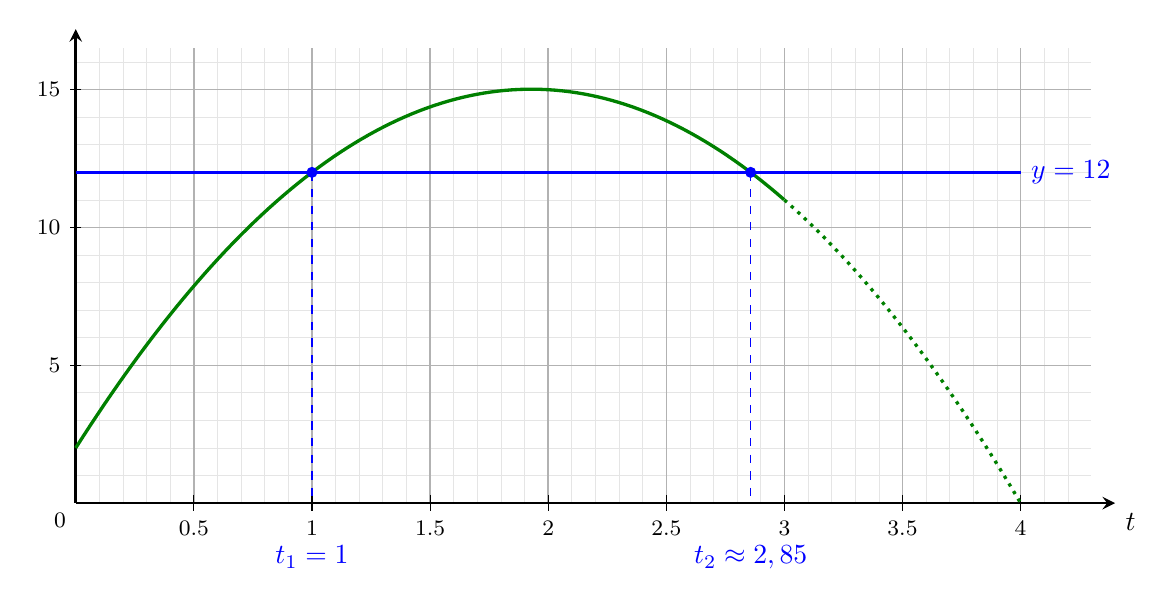
\begin{tikzpicture}[x=3cm,y=0.35cm,>=stealth]
			
			\draw[gray!20,line width=0.3pt,xstep=0.1,ystep=1] (0,0) grid (4.3,16.5);
			\draw[gray!60,line width=0.5pt,xstep=0.5,ystep=5] (0,0) grid (4.3,16.5);
			
			\draw[->,line width=1pt] (0,0) -- (4.4,0) node[below right]{$t$};
			\draw[->,line width=1pt] (0,0) -- (0,17.2);
			
			\foreach \x in {0.5,1,1.5,2,2.5,3,3.5,4} \draw (\x,3pt) -- (\x,-3pt) node[below]{\footnotesize \np{\x}};
			\foreach \y in {5,10,15} \draw (2pt,\y) -- (-2pt,\y) node[left]{\footnotesize \np{\y}};
			\draw (0,0) node[below left]{\footnotesize 0};
			
			\draw[green!50!black,line width=1.2pt,domain=0:3,samples=100]
			plot (\x,{-3.5*(\x)^2+13.5*\x+2});
			\draw[green!50!black,line width=1.2pt,dotted,domain=3:4,samples=40]
			plot (\x,{-3.5*(\x)^2+13.5*\x+2});
			
			\draw[blue,line width=1pt] (0,12) -- (4,12) node[right]{$y=12$};
			
			\draw[blue,dashed] (1,12) -- (1,0);
			\draw[blue,dashed] (20/7,12) -- (20/7,0);
			\fill[blue] (1,12) circle(2pt);
			\fill[blue] (20/7,12) circle(2pt);
			\draw[blue] (1,0) node[below,yshift=-12pt]{$t_1=1$};
			\draw[blue] (20/7,0) node[below,yshift=-12pt]{$t_2\approx 2,85$};
		\end{tikzpicture}
	\end{center}
	
Les solutions sont
		\[t_1 = 1 \qquad\text{et}\qquad t_2  \approx 2,85.\]

La hauteur du projectile est supérieure ou égale à 12~m sur l'intervalle de temps $[1 ; 2,85]$ (en secondes).

		\item Le projectile touche le sol lorsque sa hauteur s'annule :
		\[f(t) = 0 \iff (2-0,5t)(7t+1) = 0 \iff 2-0,5t = 0 \text{ ou }7t+1=0.\]
		\[ \iff -0.5t = -2 \text{ ou } 7t = -1\]
		\[ \iff t = 4 \text{ ou } t = -\frac{1}{7}\]
		
		Seule la solution $t = 4$ appartient à l'intervalle $[0~;~+\infty[$.

		Le projectile touche le sol 4~secondes après son lancement.
	\end{enumerate}
\end{enumerate}
